\documentclass{beamer}
\usepackage[utf8]{inputenc}
\usepackage{graphicx}
\usepackage{xcolor}
\usepackage{listings}
\usepackage{tikz}
\usepackage{graphicx}

\graphicspath{ {./figs/} }
\usetikzlibrary{fit}

\hypersetup{
    colorlinks=true,
    urlcolor=cyan
}

\title{Bubble Detection}
\author{Filip Peterek}
\institute{V\v{S}B-TUO}
\date{September 2024}

\begin{document}

\frame{\titlepage}

\section{Bubble Detection}

\begin{frame}
    \frametitle{Dataset}

    \begin{itemize}
        \item Dataset from CAS
        \item Manual annotation was necessary
        \item Original dataset contains noise, blurry bubbles
        \item Only bubbles recognizable by human eye are considered
        \begin{itemize}
            \item More than a couple pixels in diameter
            \item Not too blurry
        \end{itemize}
    \end{itemize}

\end{frame}

\begin{frame}
    \frametitle{First Training Set}

    \begin{itemize}
        \item Bounding boxes around bubbles
        \item Training set consists of 16 images containing 2766 bubbles
        \item Testing set consists of 2 images containing 509 bubbles
        \item Used to train RCNNs
    \end{itemize}

\end{frame}

\begin{frame}
    \frametitle{Second Training Set}

    \begin{itemize}
        \item Singular bubbles were extracted
        \item Roughly 2500 images of singular bubbles
        \item Roughly 2000 images of smidges, noise or clusters of bubbles
        \item Used to train Tsetlin Machines
    \end{itemize}

\end{frame}

\begin{frame}
    \frametitle{RCNN Detection}

    \begin{itemize}
        \item Faster RCNNs were used for bubble detection
        \item Resnet-50-FPN
        \item Transfer learning was applied
        \item Has trouble detecting very small bubbles
        \item Sometimes misses overlapping bubbles
        \begin{itemize}
            \item When both bubbles are very dark
            \item Hardly recognizable even by human eye
        \end{itemize}
        \item Couldn't suffice by itself
        \item Adjusting contrast improved detection
    \end{itemize}

\end{frame}

\begin{frame}
    \frametitle{Segmentation and Tsetlin Machines}

    \begin{itemize}
        \item To catch what RCNN missed, segmentation is used
        \item First, contrast is adjusted
        \item Then, thresholding is applied
        \item Simple flood fill algorithm selects objects in image
        \item Histogram of oriented gradients is computed for each object
        \item Tsetlin Machine then determines whether object is a singular bubble
    \end{itemize}

\end{frame}

\begin{frame}
    \frametitle{Combining Results}

    \begin{itemize}
        \item RCNN and Segmentation results are merged together
        \item Intersection over union is computed
        \item If IOU for two objects passes a certain threshold, we consider them the same object
        \item Thus, duplicates are filtered
        \item Segmentation results are preferred over RCNN results
        \begin{itemize}
            \item Prevents margins around bubbles
        \end{itemize}
    \end{itemize}

\end{frame}

\begin{frame}
    \frametitle{Results}

    \begin{itemize}
        \item Around TODO accuracy
        \item Detection using Resnet takes TODO ms
        \item Recognition using Tsetlin Machines takes TODO ms
        \item In total, processing one image takes TODO ms
        \item Mainly the result of an inefficient flood fill algorithm
        \item Written in Python, can by optimized
    \end{itemize}

\end{frame}

\begin{frame}
    \frametitle{Results}
    \begin{center}
        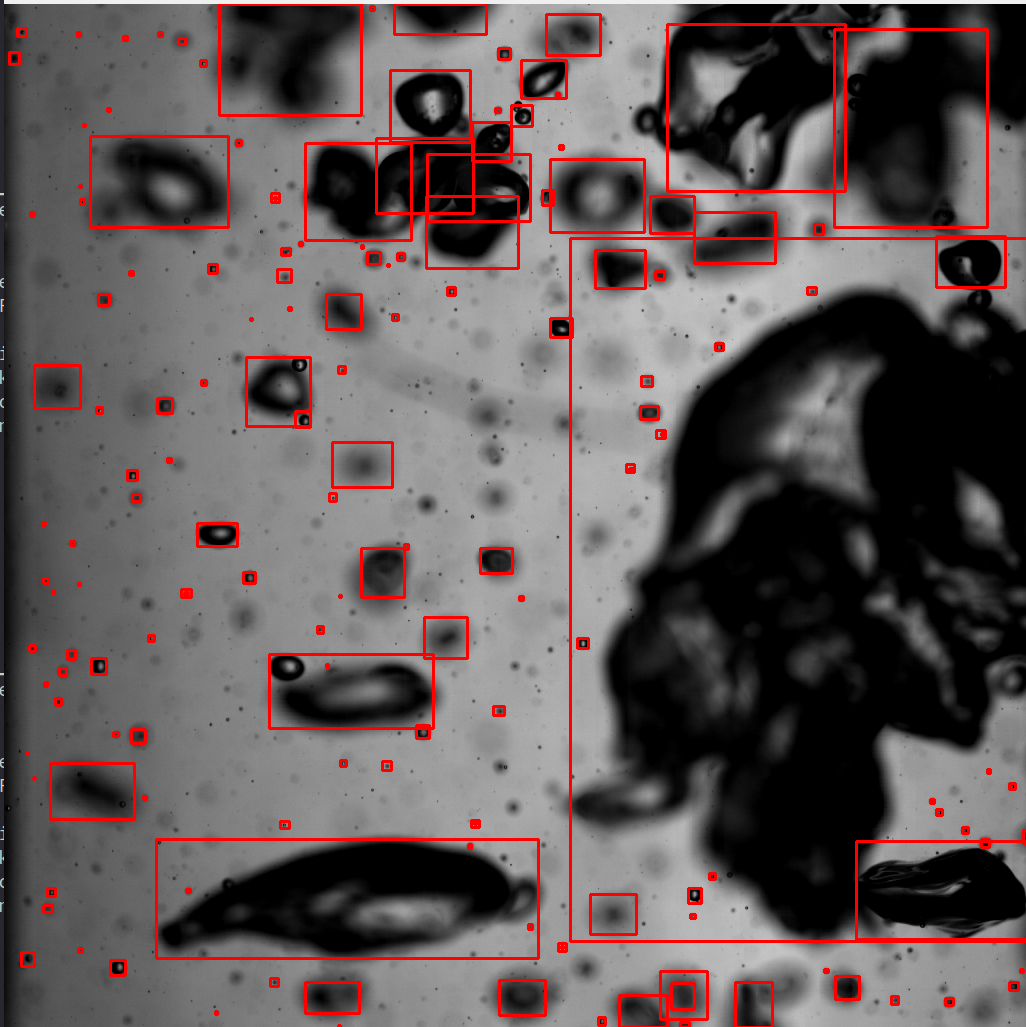
\includegraphics[width=0.8\columnwidth]{bubble-detection}
    \end{center}
\end{frame}

\begin{frame}
    \frametitle{Results}
    \begin{center}
        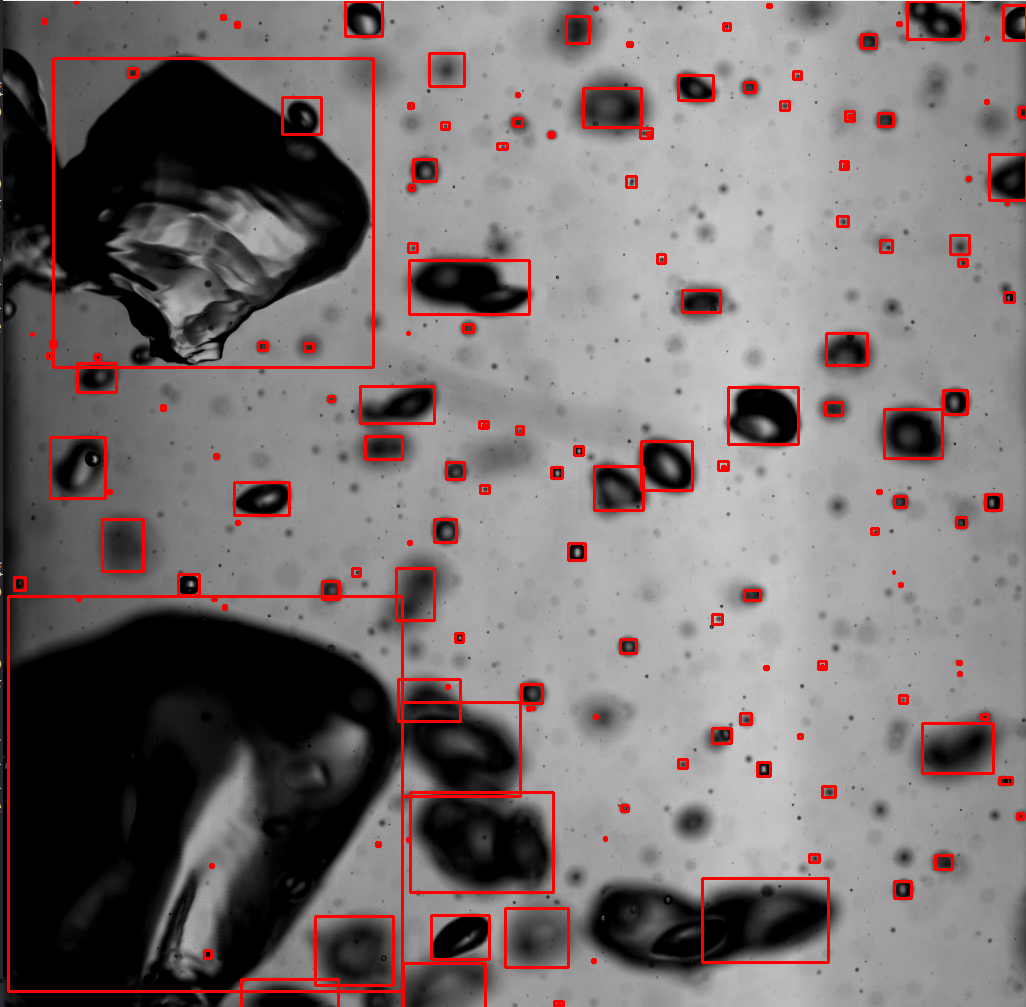
\includegraphics[width=0.8\columnwidth]{bubble-detection-2}
    \end{center}
\end{frame}

\begin{frame}
    \frametitle{Failed Experiments}

    \begin{itemize}
        \item Local Binary Pattern
        \item Background subtraction
        \item Convolutional Tsetlin Machine
    \end{itemize}

\end{frame}

\end{document}
